\section{Signal and background modelling of \texorpdfstring{\mgg}{myy}}
\label{sec:signalbackgroundmodelling}
The numbers of signal and background events in data are estimated with a fit to the \mgg spectrum as described in Section~\ref{sec:signalyieldextraction}. The functional form used to model the signal component is described in Section~\ref{ssec:signal_model}.
The forms used for the background are described in Section~\ref{ssec:background_model}.

\subsection{Signal Modelling}
\label{ssec:signal_model}
The \mgg distribution for the signal process $pp\rightarrow H \rightarrow\gamma\gamma$ is resonant.
In the absence of interference with the $pp\rightarrow\gamma\gamma$ background process this is expected to follow a Breit-Wigner curve, which peaks at the Higgs mass $m_H$ and in the Standard Model has a narrow width of $4~\text{MeV}$.
However, the distributions observed in data are smeared by the finite resolution of the measured photon energies.
For this reason, the \mgg distribution is modelled by fitting a double-sided Crystal Ball to the MC simulation with ${m_H = \SI{125}{\GeV}}$.
%% described in the common note\CiteCommon.
The analytic form of this function is presented in Eq.~\ref{E. DSCB}
\begin{equation}
  \begin{aligned}
    CB(\mgg) = N \times
    \begin{cases}
      e^{-t^{2}/2}, & \text{if } -\alpha_\text{low} \leq t \leq \alpha_\text{high} \\
      e^{-{}^{1}_{2} \alpha_\text{low }^{2}} \Big[ \frac{1}{R_\text{low}} \big(R_\text{low} - \alpha_\text{low} - t \big) \Big]^{-n_\text{low}},     & \text{if } t < -\alpha_\text{low} \\
      e^{-{}^{1}_{2} \alpha_\text{high}^{2}} \Big[ \frac{1}{R_\text{high}} \big(R_\text{high} - \alpha_\text{high} - t \big) \Big]^{-n_\text{high}}, & \text{if } t > \alpha_\text{high} \\
    \end{cases}
    \label{E. DSCB}
  \end{aligned}
\end{equation}

where $t=(\mgg-\mu_\text{CB})/\sigma_\text{CB}$, $R_\text{low}=\frac{\alpha_\text{low}}{n_\text{low}}$, and $R_\text{high}=\frac{\alpha_\text{high}}{n_\text{high}}$.
Here $N$ is a normalization parameter, $\mu_\text{CB}$ is mean of the Gaussian distribution, $\sigma_\text{CB}$ is the width of the Gaussian distribution, $\alpha_\text{low}$ and $\alpha_\text{high}$ are the positions of the transitions from the Gaussian core to the exponential tails on the low and high mass sides, and $n_\text{low}$ and $n_\text{high}$ are the exponents of the low and high mass tails.An example of this shape is shown in Figure~\ref{F. DSCB}.
The shape parameters are common to all processes ($ggH$, $VBF$, $VH$, $ttH$, $bbH$), and a fit to the sum of all processes normalised to their expected SM yield is performed for each inclusive region or bin of the differential variables.

\begin{figure}[htb!]
  \begin{center}
    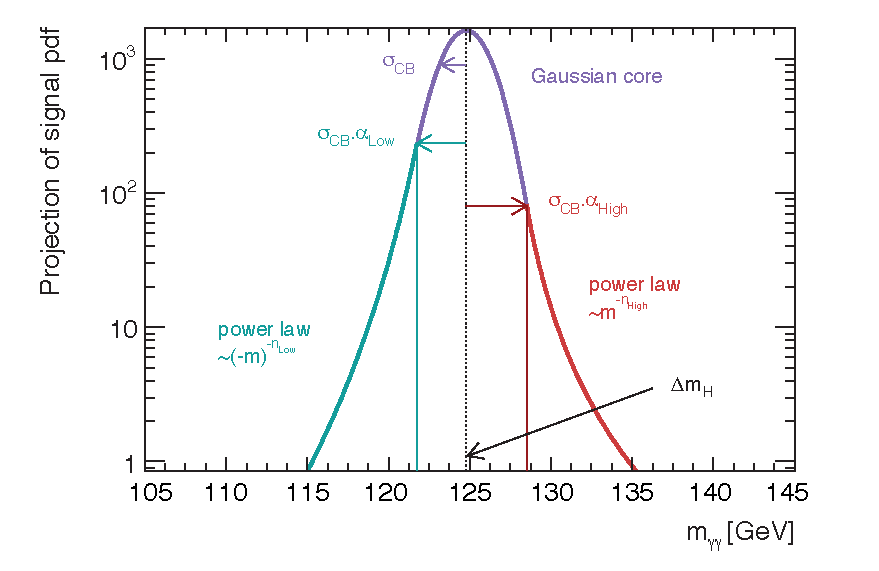
\includegraphics[width=0.48\textwidth]{figures/signal_modeling/DSCB.pdf}
  \end{center}
  \caption{Example of a double-sided crystal ball function.}
  \label{F. DSCB}
\end{figure}

Each of the shape parameters is determined by performing a fit to simulated ${H\to\gamma\gamma}$ decays at ${\mgg=\SI{125}{\GeV}}$.
In order to simulate a Higgs boson with a mass of 125.09\,\GeV, the resulting $\mu_\textrm{CB}$ will be shifted by 90\,\MeV.
This value is then fixed in the signal extraction fit and can vary for the different bins.
Shifts in $\mu_\textrm{CB}$ are still allowed through uncertainties taken into account as nuisance parameters in the fit, described in the next section.
This parametrisation is derived separately for each bin (aka category) of the variable in question.
Figures~\ref{fig:sig_model_Diphoton_fid} show an example of fits for the inclusive fiducial volume.
Signal modelling plots for the other fiducial volumes and for the differential variables are shown in Appendix \ref{app:signal_fit}.
\begin{figure}[htb!]
  \begin{center}
    \subfloat[Diphoton Fiducial]{\includegraphics[width=0.5\textwidth]{figures/signal_modeling/fit_plots_Diphoton_fid_bin1.png}}
  \end{center}
  \caption{Signal parametrisation for the inclusive fiducial volume normalised to 168~\ifb}
  \label{fig:sig_model_Diphoton_fid}
\end{figure}

\subsection{Background Modelling }
\label{ssec:background_model}

The main backgrounds in this analysis are non-resonant continuum backgrounds from inclusive $\gamma-\gamma$, $\gamma-jet$ and $jet-jet$ events.
These have smoothly falling distributions and are described by an empirically chosen functional form.
This may cause an increase (or decrease) in the measured signal events, so the selection is based on picking the function separately for each bin which reduces this bias, as described in Section~\ref{ssec:Spurious signal}.
Several functional forms for parametrization of the diphoton mass spectrum background were considered: exponentials of first (Exp), second (ExpPoly2), and third (ExpPoly3) degree polynomials, Bernstein polynomials of degree 3 (Bern3), 4 (Bern4), and 5 (Bern5) and power law functions of first (Pow)  order.
Previous studies \cite{ATLAS_prevNote} showed that the best function to model the background distribution in most cases is ExpPoly2:
\begin{equation}
  \mathcal{B}\left(\mgg;\textbf{$\alpha^\text{bkg}$}\right) = N\left(\textbf{$\alpha^\text{bkg}$}\right) \cdot \exp \left( - \frac{\mgg}{\alpha_1^\text{bkg}} - \frac{m_{\gamma\gamma}^2}{\alpha_2^\text{bkg}} \right)
\end{equation}
where $\alpha^\text{bkg}_{1}$, $\alpha^\text{bkg}_{2}$ are nuisance parameters and $N\left(\textbf{$\alpha^\text{bkg}$}\right)$ normalises the function to unity.
In general, a higher-order exponential is needed for bins with more events.

The Bernstein polynomials of degree $n$ are defined as:
\begin{equation}
   \mathcal{B}\left(\mgg;\textbf{$\alpha^\text{bkg}$}\right) = N\left(\textbf{$\alpha^\text{bkg}$}\right) \cdot
   \sum_{i=0}^n \alpha^\text{bkg}_i x^{i} \cdot (1 - x)^{n-i} \cdot \frac{n!}{i! \cdot (n-i)!}
\end{equation}

where $x = \frac{\mgg-\mgg^\textrm{min}}{\mgg^\textrm{max}-\mgg^\textrm{min}}$ is a variable defined in the range $[0,1]$ and $\alpha^\text{bkg}_0=1$.

For the power law function, the first order (Pow) is defined as

\begin{equation}
  \mathcal{B}\left(\mgg;\textbf{$\alpha^\text{bkg}$}\right) = N\left(\textbf{$\alpha^\text{bkg}$}\right) \cdot m_{\gamma\gamma}^{\alpha_1}
\end{equation}


\FloatBarrier
\subsubsection{Background template}
\label{ssec:Background template}
Due to computational limitations only the $\gamma\gamma$ sample is generated, the contribution of $\gamma j$ and $jj$ component are derived from data using a two-dimensional
double-sideband method as described in section \ref{sec:backgroundestimation}.The fraction of contributed by the $\gamma\gamma$,$\gamma j$ and $jj$ background source after inclusive diphoton selection are 67\%,29\% and 4\% respectively. In previous note ~\cite{ATLAS_prevNote}, it was studied that using only $\gamma\gamma$ and $\gamma j$ components for modelling the shape, a good description of the background in the data sideband can be achieved and the $jj$ contribution can be neglected.The $\gamma j$ shape is derived from data control region. In the control region. The events should pass the LoosePrime4 working point and the tight identification for one of the two photon candidates is inverted.Then the shape is smoothed by fitting its ratio to the $\gamma\gamma$ MC shape with a smooth function and apply the reweighting to $\gamma\gamma$ MC shape.An illustration for this procedure is shown in Figure~\ref{fig:yj_CR_inclusive} for the di-photon inclusive region. 

\begin{figure}[!htbp]
	\begin{center}
\includegraphics[width=0.45\textwidth]
      {figures/BackgroundTemplates/yjbkg_Diphoton_fid_bin0.png}
	\end{center}
	\caption{Control region plot for the inclusive selection. The $\gamma$--jet data from the control region are reweighing using $\gamma\gamma$ MC according to its ratio to $\gamma\gamma$ MC. The ratio is fitted with a smooth function.}
	\label{fig:yj_CR_inclusive}
\end{figure}

The total background shape is the addition of $\gamma\gamma$ and $\gamma j$ according to the relative fractions.The total background template is build by normalized the shape to match the data entries in the sideband range(i.e. excluding 121 \GeV <\mgg< 129 \GeV).The uncertainties are derived from $\gamma\gamma$ MC statistical uncertainties.The templates show a good agreement when comparing with the events in data sidebands.As shown in Figure ~\ref{fig:data_sideband_inclusive}
\begin{figure}[!htbp]
	\begin{center}
\includegraphics[width=0.45\textwidth]
      {figures/BackgroundTemplates/MC_Data_Diphoton_fid_bin0.png}
	\end{center}
	\caption{comparison plot between template and data sideband}
	\label{fig:data_sideband_inclusive}
\end{figure}

\subsubsection{Background smoothing}
\label{ssec:background smoothing}
Due to the finite size of the simulation samples used to build the background templates,
large statistical fluctuations are often observed. These fluctuations can adversely affect
the estimation of the spurious signal, particularly when they occur in the Higgs signal
window between 123\GeV and 127 \GeV. These fluctuations would nominally be interpreted
as a spurious signal, hence resulting in an overestimation of the background model’s
systematic uncertainty. Given the computational limitations in generating larger data
sets, an alternative approach is employed. The background templates are smoothed using
Gaussian process regression (GPR) ~\cite{frate2017modelingsmoothbackgroundsgeneric}. The GPR smoothing is performed using the Scikit-Learn machine learning package.In the GPR smoothing, the Gibbs kernel is used, which is based on the commonly used Radial Basis Function (RBF) kernel\cite{Berger:2764716}.
The RBF kernel has one hyperparameter, the constant length scale $l$, and it is defined as

\begin{equation}
K_\text{RBF}(x,x') = exp\left(\frac{-(x-x')^2}{2l^2}\right)
\end{equation}

The RBF kernel is useful for mostly-flat functions. However, for smoothly-falling functions, it is likely that nearby points will be more correlated in some regions than in others, so a constant length scale is a suboptimal model. The Gibbs kernel allows the length scale $l(x)$ to vary linearly as a function of $x$, and thus has two hyperparameters: the initial length scale and the length scale slope. The Gibbs kernel function is: 

\begin{equation}
K_\text{Gibbs}(x, x') = \frac{\sqrt{2l(x)l(x')}}{l(x)^2 + l(x')^2 } \cdot exp\left( \frac{-(x-x')^2}{l(x)^2 + l(x')^2} \right)
\end{equation}

The background templates used in the spurious signal test for the analysis categories are all smooth,roughly exponentially falling distributions with statistical fluctuations.hence the Gibbs kernel and an additional custom error kernel is used.For the error kernel.the magnitude of the errors decrease linearly with x.The two hyperparameters -- $\epsilon$ and $\epsilon_{b}$ --are highly constrained to approximate the error bars from the original background template.

Large data statistical fluctuation may cause problems with GPR fit convergence.The GPR prior is used to provide a very rough approximation of the background shape.The prior is usually defined by fitting the background template with  an exponential function. However, in cases where the input template has very few statistics.The GPR fit almost unchanged with the exponential prior.Although the exponential shape is technically an adequate descriptor of the template shape, the choice of the exponential mean does bias the functional choice of the spurious signal test in this case.Therefore, a check has been added to re-perform the GPR fit using a flat prior if the GPR fit and exponential prior disagree with $\frac{\chi^2}{ndf} <1$.

The smoothed template shows good agreement with both the raw template and the data sidebands, as illustrated in the left plots of Fig.~\ref{fig:template_inclusive}. The right plots present a comparison of the templates before and after smoothing. A $\chi^2$ test is performed to evaluate the compatibility between the raw and smoothed templates. In the lower panel of the right plot, the pull distribution, defined as $\frac{MC - \text{GPR}}{\sigma_{MC}}$ is shown and varies mostly within $1\sigma$. For more template plots can be found in Appendix\ref{app:bkg_template}

\begin{figure}[htbp!]
  \begin{center}
    \subfloat[]{\includegraphics[width=0.45\textwidth]{figures/BackgroundTemplates/DataSB_Diphoton_fid_bin0.png}}
    \subfloat[]{\includegraphics[width=0.45\textwidth]
    {figures/BackgroundTemplates/Smoothed_Diphoton_fid_bin0.png}}\\
  \end{center}
  \caption{(a) comparison plot for background templates and data sidebands for inclusive region. (b) compatibility check plot between raw template and smoothed template.}
  \label{fig:template_inclusive}
\end{figure}



\subsubsection{Spurious signal Test} 
\label{ssec:Spurious signal}

The spurious signal method is used to measure the bias in the signal yield caused by the choice of background parameterisation.
This is done by fitting a background only MC simulation with a signal + background parameterisation. 


The signal yield extracted in the background-only template (S) and its statistical uncertainty ($\Delta_{\textrm{S}}$) are used to measure the bias introduced by the choice of the background parametrisation. The condition of a function to be accepted is that either:

\begin{itemize}
	\item S  is less than 20\% of the background uncertainty
	\item S  is less than 10\% of the number of expected signal events.
\end{itemize}


The mass range of 123-127\,\GeV\ is split into  bins with a 0.5\,\GeV\ width and the maximal signal found in these bins is taken as spurious signal.
 
In case several functions satisfy the above criteria, the one with fewest degree of freedom is chosen. If two such functions are found , the one with the lower spurious signal uncertainty is taken. 
 
Furthermore, an additional  $\chi^2$ probability ensures that the side-bands from the  MC templates are also described well requiring that the $p$-value is larger than 1\%.
This $p$-value is evaluated on the un-smoothed template.For the template changed due to the $p$-value. the corresponding bins are labelled with "p($\chi^{2}$) change". 
 For all past functions with a lower $p$-value, dedicated toy studies are performed to verify that the selected background function is a good choice. The corresponding bins are labeled with "toy studies" and the detail explanation in \cite{HIGG-2019-13-INT1}.currently no corresponding bins for this case.

 The function choice and the evaluation of the spurious signal is evaluated on the GPR smoothed template in order to reduce the effect of statistical fluctuations on this uncertainty.

 Additional studies were performed for analysis bins, where the agreement between the data sideband and the un-smoothed background template did not look good. Overall, the studies showed that no extra treatment for those bins is needed as the effect on the spurious signal is negligible for bins where the  selected function has at least two degrees of freedom\cite{HIGG-2019-13-INT1}. There was only one bin (\mjj bin 5) with a bad data/MC agreement(p($\chi^{2})<1\%$) where a function with one degree of freedom was selected. In this case, it was found by a "manual F-test", that the function of two degrees of freedom is preferred.

In the case of bins with low statistics, an Exponential function is used. A bin is considered as low statistics, if the background template has at least one bin with less than 20 effective events\footnote{GPR smoothing assumes that each bin follows Gaussian statistics, which is not true for low statistics bins which follow Poisson statistics.where the effective events $N_{eff}=(\frac{bin_{content}}{bin_{error}})^{2}$}.
This corresponds to bins where less than 150 data events from the sideband region are expected.This choice of the Exponential function is validated based on a Wald test on the data-sidebands. Furthermore no GPR smoothing is applied. Those bins are labelled with "low stat". Only the last two bins of \ptgg have low statistical bins.However,For the lepton category, low statistics are also observed due to missing Monte Carlo background samples (e.g. $V\gamma\gamma$, $t\bar{t}\gamma\gamma$). No special treatment is applied to this category in the spurious signal procedure, instead, it is labeled as “MC sample missing.”
 
For the bins which observed that background function choice was Pow, while in the F-tests, it was seen that Pow and Pow2 are both failing the test and at least a Pow3 function would be needed. In this case, the Pow family does not seem to be a reliable estimate. An Exponential function performed similar good and no further changes from the F-test are required, so it was decided to use Exponential instead. The bins are labelled with "F-test".
currently no corresponding bins for this case.

The functional form and spurious signal uncertainties for each fiducial volume and each analysis bin are estimated independently.Therefore the resulting spurious signal uncertainties are uncorrelated across bins.

The selected background functions are summarized for all analysis bins in \ptgg in Table~\ref{tab:sp_signal_pT_yy_main}. The detailed information for all other variables can be found in Appendix~\ref{app:spurious_signal}.

For each analysis bin, the selected function is given. In the next column, the spurious signal uncertainty is given. This uncertainty is evaluated from the maximal spurious signal in the bin (and given in the next column) divided by the reference signal (based on MC). In the next column, the spurious signal is given, followed by the spurious signal relative to the expected statistical uncertainty on the signal. The last column indicates the selection criteria, 'toy studies', 'low stat' or 'manual F-test' in case of a special treatment of the bin . Furthermore, it is indicated if a change of function is required due to the F-test (see Section~\ref{ssec:wald-test}). In this case, the spurious signal and the corresponding uncertainty before the function change is given in parentheses.

\begin{table}[htbp!]
\centering
\caption{Spurious signal results for all analysis bins for \ptgg}
\label{tab:sp_signal_pT_yy}
\begin{tabular}{lrrrrc}
\toprule
Variable bins & Sel.Func & SS[\%] & max(S) & $S/S_{ref}$[\%] & criteria \\
\midrule
$0 \leq \ptgg < 5$\GeV & ExpPoly2 & -1.83 & -4.94 & -3.64 &  \\
$5 \leq \ptgg < 10$\GeV & ExpPoly2 & -2.32 & -17.2 & -8.97 &  \\
$10 \leq \ptgg < 15$\GeV & ExpPoly3 & -6.25 & -44.4 & -20 & F-test(-6.02,-44.9) \\
$15 \leq \ptgg < 20$\GeV & ExpPoly2 & -5.61 & -35 & -18.9 &  \\
$20 \leq \ptgg < 25$\GeV & ExpPoly2 & -9.15 & -49.7 & -27.7 &  \\
$25 \leq \ptgg < 30$\GeV & ExpPoly2 & 2.26 & 12.9 & 7.64 &  \\
$30 \leq \ptgg < 35$\GeV & ExpPoly3 & 5.6 & 27.2 & 14.6 &  \\
$35 \leq \ptgg < 45$\GeV & ExpPoly2 & 4.54 & 35.4 & 18.9 &  \\
$45 \leq \ptgg < 60$\GeV & ExpPoly2 & -2.42 & -20 & -11.5 &  \\
$60 \leq \ptgg < 80$\GeV & ExpPoly3 & -1.44 & 0 & 0 & $p(\chi^2)$ change \\
$80 \leq \ptgg < 100$\GeV & Bern3 & 6.62 & 28.4 & 25.3 &  \\
$100 \leq \ptgg < 120$\GeV & Pow & 3.72 & 10.2 & 14.8 &  \\
$120 \leq \ptgg < 140$\GeV & ExpPoly2 & 1.75 & 2.85 & 5.53 & F-test(-1.13,-1.98) \\
$140 \leq \ptgg < 170$\GeV & Exponential & -3.33 & -6.38 & -15.9 &  \\
$170 \leq \ptgg < 200$\GeV & Exponential & -0.207 & -0.222 & -0.829 &  \\
$200 \leq \ptgg < 250$\GeV & Exponential & 1.26 & 1.23 & 5.43 &  \\
$250 \leq \ptgg < 300$\GeV & Exponential & 1.12 & 0.547 & 4.11 &  \\
$300 \leq \ptgg < 450$\GeV & Exponential & -0.817 & -0.341 & -3.23 &  \\
$450 \leq \ptgg < 650$\GeV & Exponential & 4.04 & 0.325 & 8.06 & low stat \\
$650 \leq \ptgg < 13000$\GeV & Exponential & 2.25 & 0.0335 & 2.15 & low stat \\
\bottomrule
\end{tabular}
\end{table}



\subsubsection{Wald tests} 
\label{ssec:wald-test}
Because data might contain features not found in MC simulation, an additional test is done on the data-sidebands to check if a higher-order function is needed.
The functional form of the background selected by the spurious signal method is confronted with a Wald test (also named as F-test).
The data from 2022-2024 sidebands, excluding 120--130~\GeV, were used to test the hypothesis that additional degrees of freedom for the chosen fit function is not needed to accurately describe the data.

The test statistic that is used for this test is defined as
\begin{equation}
	\lambda_{(1,2)} = -2\ln(L_1/L_2)
\end{equation}
where $L_1$ and $L_2$ are the likelihood values of the two fits,
that with the nominal background model and that with a model with
an additional degree of freedom. The test statistic has an asymptotic
distribution of a $\chi^2$ variable with one degree of freedom.

The additional parameter is deemed necessary if
$P(\lambda_{(1,2)}' \geq \lambda_{(1,2)}) < 0.05 $, where $P$ is the probability
of observing a $\lambda_{(1,2)}'$ value higher than the observed one.
In this case the, nominal model becomes the one with an extra degree of freedom,
which in turn is tested against a model with one more d.o.f. and so on
until $P(\lambda_{(1,2)}' \geq \lambda_{(1,2)}) > 0.05$. The wald test plot results are shown in \ref{app:sideband_wald_test}.

The results of this test are summarised in Table~\ref{tab:f_test_results} for all bins failing the test and where therefore the background function and corresponding spurious signal results used for the analysis are changed. This introduced in addition to the already tested functions, an Exponential with fourth degree of freedom and also an increase of degree of freedom for the Pow function (Pow2).
\begin{table}[htbp!]
    \centering
    \begin{tabular}{ c |c c| c c}
        \hline
        Variable bins & Func. & SS [\%] & New Func. & new SS [\%] \\
        \hline
         VBF-enhanced                & ExpPoly2 &  1.4  & ExpPoly3 & -0.731 \\
         $15 \leq \ptgg < 20$\GeV   & ExpPoly2 & -6.02 & ExpPoly3 & -6.25 \\
         $120 \leq \ptgg < 140$\GeV  & Exponential & -1.31 & ExpPoly2 &  1.75 \\
         $0.9 \leq \ygg < 1.2$       & ExpPoly2 & -5.35 & ExpPoly3 & -5.75 \\
        \hline
    \end{tabular}
    \caption{F-Test results for all analysis bins.}
    \label{tab:f_test_results}
\end{table}